\begin{frame}
	\frametitle{Fitness function}
	
	\begin{columns}[c]
		
		\column{.45\textwidth}

		\begin{itemize}
			\item function for e.g. branch distance
			\item guidance for search algorithms
		\end{itemize}
		
		\begin{figure}
			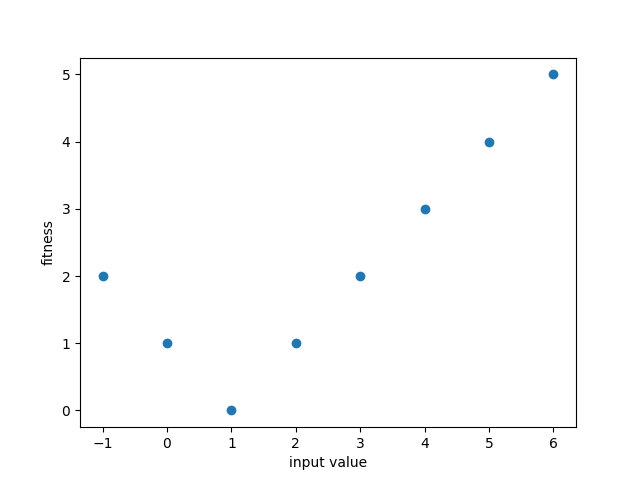
\includegraphics[width=1\textwidth]{figures/plot_guidance}
		\end{figure}
		
		\column{.45\textwidth}
		\lstinputlisting{code/simple_guidance.java}

	\end{columns}
	
\end{frame}

\begin{frame}
	\frametitle{Fitness landscape}
	
	\begin{columns}[c]
		
		\column{.45\textwidth}

		\begin{itemize}
			\item metaphor for the search space
			\item fitness value as height
			\item input as depth and width
			\item search for minima
		\end{itemize}
		
		\column{.45\textwidth}
		\begin{figure}
			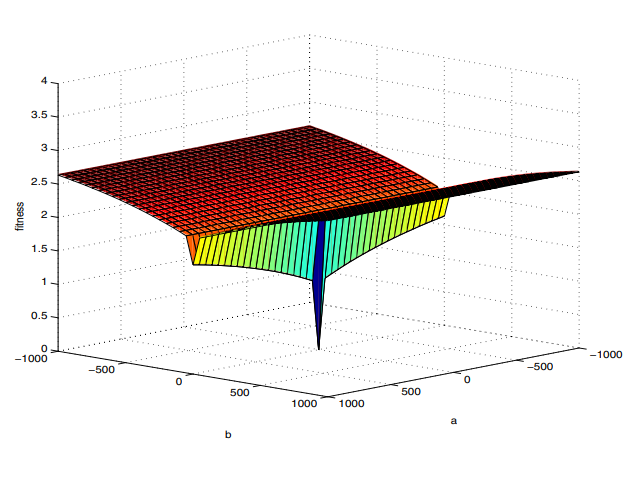
\includegraphics[width=1\textwidth]{figures/complex_landscape}
		\end{figure}
		\cite{Harman.2007}
		
	\end{columns}
	
\end{frame}

\begin{frame}
	\frametitle{Random Walk}
	
	\begin{columns}[c]
		
		\column{.45\textwidth}

		\begin{itemize}
			\item \cite{Kauffman.1987}
			\item used to describe landscape
			\item walk over landscape
			\item random unbiased steps
		\end{itemize}
		
		\column{.45\textwidth}
		\begin{figure}
			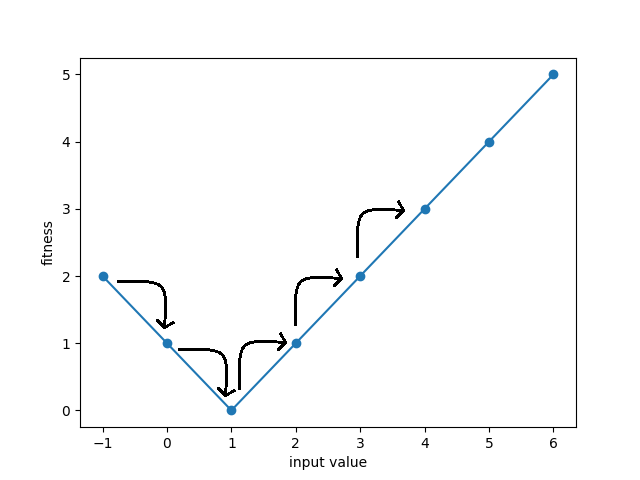
\includegraphics[width=1\textwidth]{figures/random_walk}
		\end{figure}

	\end{columns}
	
\end{frame}

\begin{frame}
	\frametitle{Long Jump}
	
	\begin{columns}[c]
		
		\column{.45\textwidth}

		\begin{itemize}
			\item \cite{Kauffman.1987}
			\item multiple steps
			\item landscape approximation
		\end{itemize}
		
		\column{.45\textwidth}
		\begin{figure}
			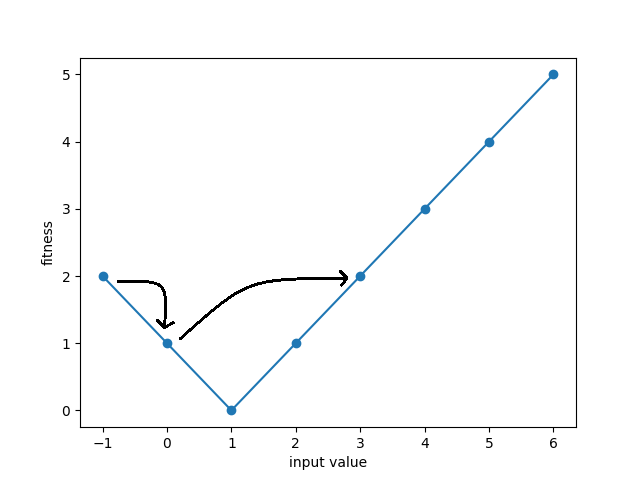
\includegraphics[width=1\textwidth]{figures/long_jump}
		\end{figure}

	\end{columns}
	
\end{frame}

\begin{frame}
	\frametitle{Genetic algorithm}
		
	\begin{itemize}
		\item test = individual
		\item multiple tests = population
		\item start with random population
		\item iterate till termination condition
		\begin{itemize}
			\item mutate and crossover
		\end{itemize}
		\item return last generation
	\end{itemize}
		
	
\end{frame}

\begin{frame}
	\frametitle{DynaMOSA}
	
	\begin{columns}[c]
		
		\column{.45\textwidth}
		
		\begin{itemize}
			\item genetic algorithm
			\item multiple target
			\item keep track of target covering individuals
			\item keep track of covering individuals (archive)
		\end{itemize}
		
		\column{.45\textwidth}
		
		\begin{itemize}
			\item dynamic target update
			\item archive update
			\item select by rank
			\item return archive as last generation
		\end{itemize}	
		
	\end{columns}
	
\end{frame}

\begin{frame}
	\frametitle{Parameter tuning and control}
	
	\begin{figure}
		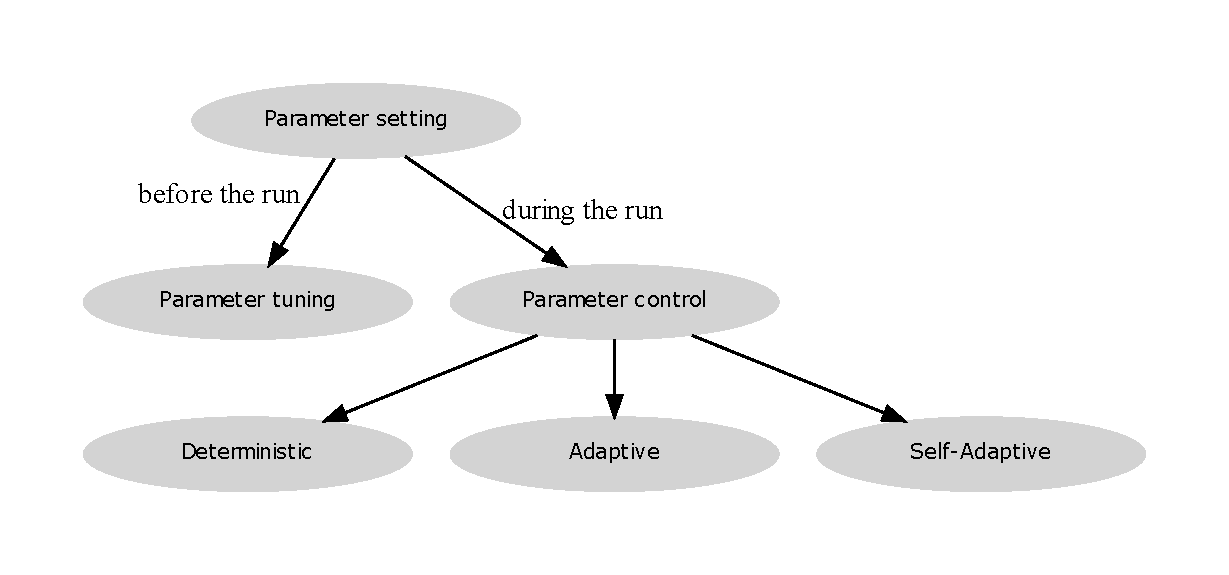
\includegraphics[width=0.9\textwidth]{figures/flowchart_parameter_control}
	\end{figure}
	\cite{Eiben.1999}
	
\end{frame}